
% JuliaCon proceedings template
\documentclass{juliacon}
\setcounter{page}{1}

\begin{document}

% **************GENERATED FILE, DO NOT EDIT**************

\title{My JuliaCon proceeding}

\author[1]{1st author}
\author[1, 2]{2nd author}
\author[2]{3rd author}
\affil[1]{University}
\affil[2]{National Lab}

\keywords{Julia, Optimization, Game theory, Compiler}

\hypersetup{
pdftitle = {My JuliaCon proceeding},
pdfsubject = {JuliaCon 2019 Proceedings},
pdfauthor = {1st author, 2nd author, 3rd author},
pdfkeywords = {Julia, Optimization, Game theory, Compiler},
}

\maketitle

To study the cosmos, astronomers use data cubes with many dimensions representing images with axes for sky position, time, wavelength, polarization, and more. Since these large datasets often span many orders of magnitude in intensity and typically include colours invisible to humans, astronomers like to visualize their images using a variety of non-linear stretching and contrast adjustments.
Additionally, images may contain metadata specifying arbitrary mappings of pixel positions to multiple celestial coordinate systems.
Julia\cite{bezanson2017julia} is a powerful language for processing astronomical data, but these visualization tasks are a challenge for any tool.

\vspace{0.2cm}
\emph{Background.}
One of the most ubiquitous data formats used in astronomy is FITS, or the Flexible Image Transport System.
Compared to a traditional raster image formats, FITS files are more like containers or small filesystems.
Each file contains one or more header data units (HDUs) that pair a dataset with a header.
The FITS format and header conventions have developed organically over several decades, first by convention,
and then in a series of papers proposing new extensions and standardizing existing behaviour now summarized in \cite{fitsstandard}.

In each HDU,
headers are stored in a plain text ASCII format and are followed by data.
The data may be in the format of an N-dimensional binary array (an ``image'' HDU),
a binary table,
or an ASCII table (``table HDUs'').

The metadata described by FITS headers are quite rich.
A header consists of \verb|KEY = VALUE / COMMENT| entries, long form \verb|COMMENT| sections,
and long form \verb|HISTORY| sections used to desrcibe the sequence of transformations used to generate the data.
FITS headers often contain several hundred header entries most of which are specific to the instrument and software packages used to record and process the data.
A subset of these are standardized and used to describe the physical units and coordinates of pixels in the image, called world coordinate system (WCS) header entries.


These WCS entries record pixel locations in one or more celestial coordinate systems including, right ascension and declination, galactic coordinates, velocity, frequency, wavelength, polarization, and more.
For most coordinate schemes, pixel coordinates are encoded using an affine transformation matrix combined with a \verb|CTYPE| specifier. Images are typically sampled regularly in the plane of a detector; however, coordinate projections are in general non-linear, and the physical coordinates of each pixel, spacings between pixels, etc. may vary across the image.
In many instances, image HDUs contain 3, 4, or even 5 dimensional data cubes, and thanks to the affine transformation matrix, moving along any one of these dimensions can shift the coordinates along the other dimesions. This point is important since it means that the full coordinates of a given pixel are needed to calculate it's physical position along any one axis.


\begin{figure}[t]
    \centerline{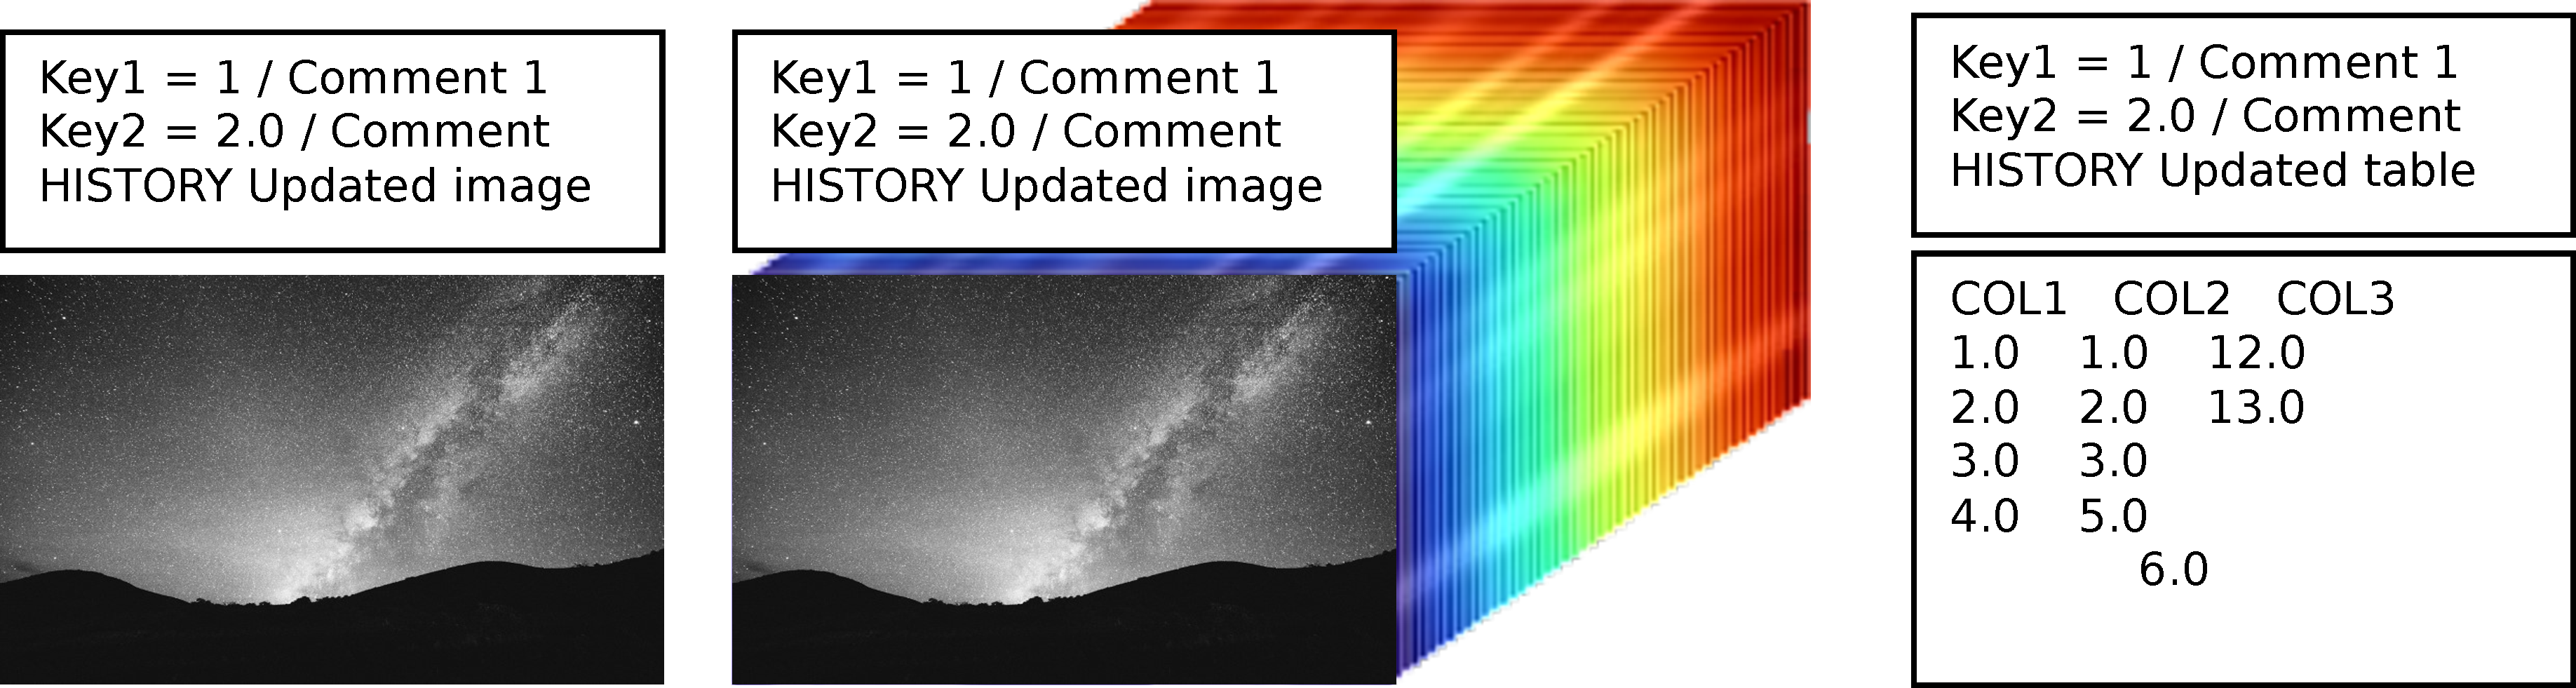
\includegraphics[width=\columnwidth]{fits-schematic.pdf}}
    \caption{Conceptual schematic of a FITS file containing a 2D image HDU, a 3D hyperspectral image HDU, and a table HDU.}
        \label{fig:fits-schematic}
\end{figure}

For image data itself, FITS files do not in general store colour information that can be displayed directly. In contrast to digital cameras, astronomical data is almost invariably captured outside the human visible range or at least with filters that are not well matched to human colour perception.
Instead, astronomers use visualizations that maps raw numerical data to a false colour image.
These steps include a linear transformation from arbitrary numerical ranges to a standard 0 to 255 display range that produces a desired contrast and brightness at an intensity level of interest.
The comparatively low dynamic range of electronic displays is often compensated for by applying non-linear mapping, or ``stretching'' such as $\log$ scales or $\mathrm{arcsinh}$ scales.
% The term ``gamma-correction'' is sometimes used to describe this step in the computer graphics community, but since matching human visual perception is less important, the stretches applied may be quite arbitrary.
Once the data is normalized to a reasonable intensity level, one typically presents a grayscale image or applies a false colour map.
Finally, one may also create a colour composite image combining multiple information layers, especially when preparing data for public consumption.

\vspace{0.2cm}
\emph{Existing Tools.}
Julia has a robust package ecosystem for loading FITS files (\verb|FITSIO.jl|), manupulating images (\verb|Images.jl| ecosystem), calculating world coordinates (\verb|WCS.jl|), and plotting (e.g. \verb|Plots.jl|).
For instance, the \verb|FITSIO| package is capable of reading and writing FITS files, headers, image HDUs, and table HDUs;
the \verb|Images| packages support generating and displaying RGB images; 
and the the \verb|WCS| package supports converting between pixel and world coordinates given a FITS header.
The Julia package ecosystem lacks, however, a package that combines these tools into a high-level interface for loading and visualizing astronomical image data.

\clearpage
\emph{The AstroImages.jl package.}
The aim of \verb|AstroImages.jl| is to tie together relevant utility packages from the Julia ecosystem to facilitate the loading, manipulation, analysis, and visualization of astronomical data.

\verb|AstroImages.jl| is registered with \verb|FileIO.jl| so that images and tables can be loaded from FITS files with the \verb|load| and \verb|save| functions.
\begin{lstlisting}[language = Julia]
using AstroImages
img = load("jwst-carina.fits")
\end{lstlisting}

\vspace{-0.4cm}
\begin{figure}[hbt!]
\centerline{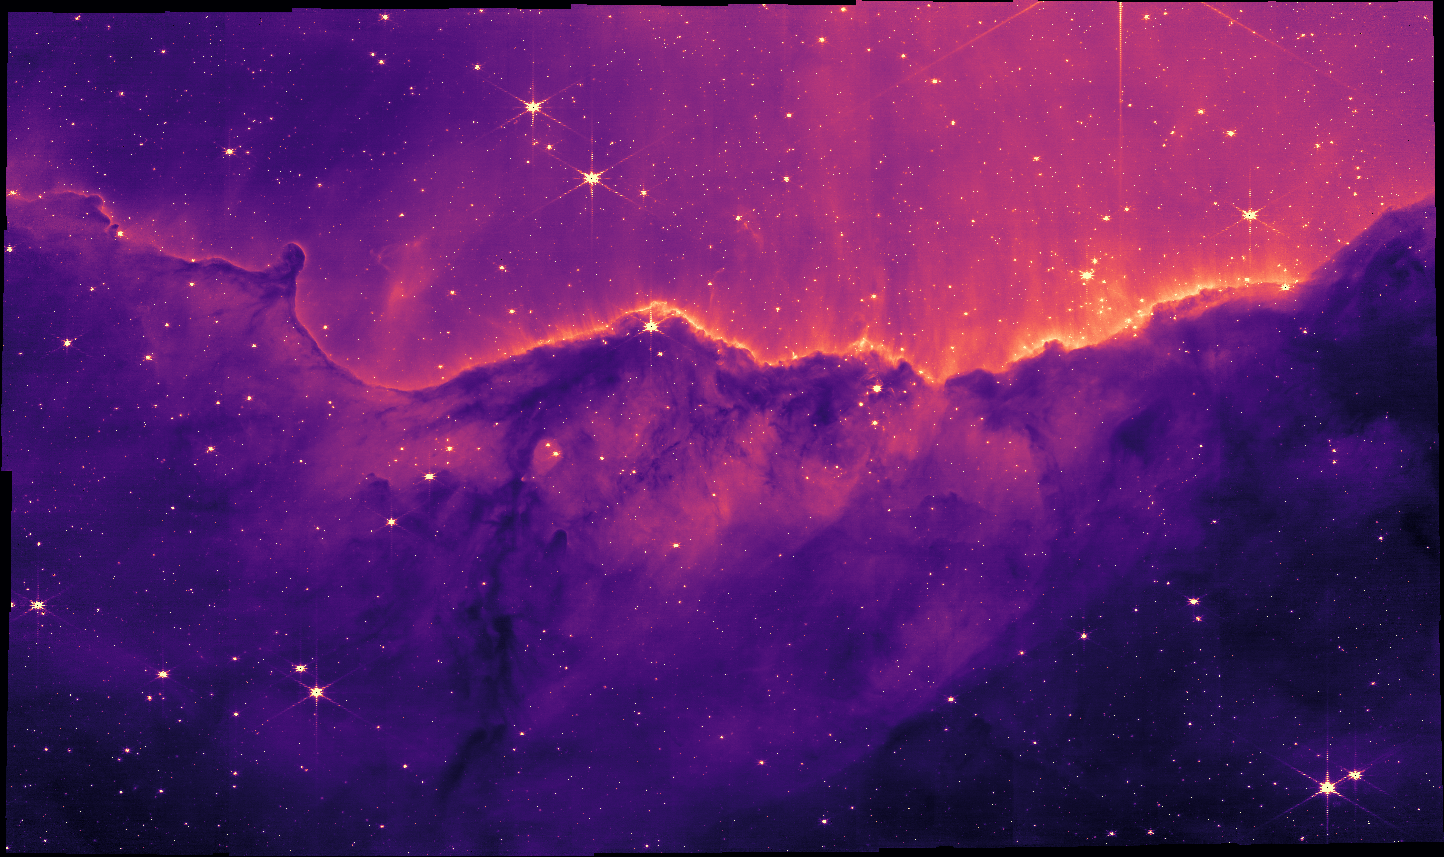
\includegraphics[width=\columnwidth]{carina.png}}
\caption{AstroImage automatically rendered as a PNG. Image of the Carina nebula from JWST commisioning data (NASA, ESA, and CSA).}
  \label{fig:jwst-carina}
\end{figure}
\FloatBarrier 

By default, this will load the first image HDU from the file. If a different HDU or a table HDU is desired, the HDU number can be passed explicitly as a second argument.
Multiple HDUs can be loaded at once by passing a tuple of HDU numbers or \verb|:|. 
% As we will see, this command will also automtically display a downscaled version of the image HDU if it is two dimensional and the user's interactive prompt supports rich output.

The values returned from \verb|load| are \verb|AstroImage| objects which combine a parent array, a FITS header, and implements the \verb|DimensionalData| \verb|AbstractDimArray| interface.
Any array type can be wrapped in an \verb|AstroImage| by passing it to the contructor.

By implementing the \verb|AbstractDimArray| interface, the dimensions of each axis of the array can be named and paired with coordinates to enable concise indexing of multi-dimensional cubes.

Once loaded, the user should be able to pass the AstroImage through any analysis code that accepts an AbstractArray. Indexing and slicing are tracked using \verb|DimensionalData.jl| so that pixel locations in the originating parent data cube are recoverable.

FITS header keys can be accessed by indexing the image with a string key, the \verb|Comment| type, and or the \verb|History| type to read and write to the header. \verb|WCS.jl| \verb|Transformation| objects can be generated using the \verb|wcs(img, wcsnum)| function and are cached unless/until the user modifies a relevant header field.

Finally, when the user wishes to display an \verb|AstroImage|, they may use either 
\verb|imview| to create a lazy mapping to RGB data or the \verb|implot| Plots.jl recipe. 
\verb|imview| accepts keyword arguments for controlling the image stretching, colour limits, colour scheme, bias, and contrast:

\begin{lstlisting}[language = Julia]
imview(img; clims=Percent(95), cmap=:magma,
    stretch=asinhstretch, contrast=1.2, bias=0.4)
\end{lstlisting}

\verb|imview| is also called automatically with configurable default values whenever an \verb|AstroImage| is displayed.
In this case, the output is automatically downscaled to a reasonable size using \verb|ImageTransformations.restrict|.
For example, all that's needed to display a 2D image HDU from a FITS file is to type \verb|load("filename.fits")| at an interactive prompt provided that prompt supports rich outputs.

The \verb|implot| Plots.jl recipe supports additional functionality. It uses \verb|imview| to first render the image and then uses Plots.jl to present an image series.

The plot recipe automatically applies WCS grid lines (which may be arbitrarily tilted and warped) and labels the axes with their coordinate types. It also creates a custom colour bar labelled with ticks at the correct, possibly non-linear spacing caused by chosen stretch.
When applied to slices of multi-dimensional cubes, \verb|implot| further titles the plot with the slice's location along the other axes.

\begin{lstlisting}[language = Julia]
using AstroImages, Plots
HIcube = load("HIdat.fits")
slice = HIcube[Z=228]
implot(slice; cmap=:turbo, stretch=asinh)
\end{lstlisting}
\vspace{-0.5cm}
\begin{figure}[hbt!]
    \centerline{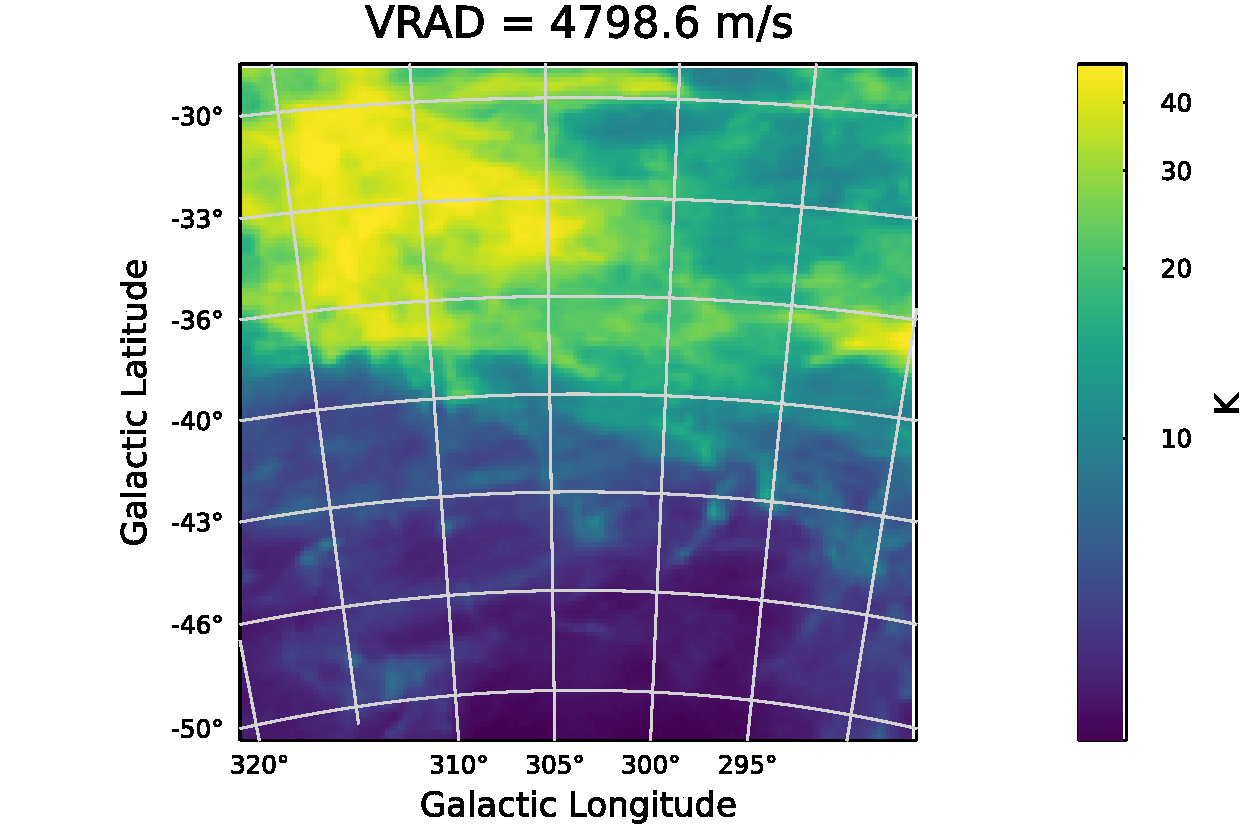
\includegraphics[width=\columnwidth]{hidatplot.pdf}}
    \caption{implot augments an image with world coordinates and automatically labelled axes, titles, and colourbar. Image is a slice through galactic latitude, longitude, and velocity space of neutral Hydrogen density (HI4PI survey \cite{2016A&A...594A.116H}).}
      \label{fig:cube-slice}
\end{figure}
\FloatBarrier 

\verb|AstroImages.jl| is a complete, high-level package for working with astronomical data in Julia.

% **************GENERATED FILE, DO NOT EDIT**************

\bibliographystyle{juliacon}
\bibliography{ref.bib}


\end{document}

% Inspired by the International Journal of Computer Applications template
